\section{Hypothesis Graph}%
\label{sec:hgraph}
The \acf{hgraph} consists of a set of nodes and edges. Where the node correspond to an object at a configuration, and the edges correspond to actions. As a whole the \ac{hgraph} represents a search in the composite configuration space. The \ac{halgorithm} creates and updates nodes and edges in the \ac{hgraph} and is discussed in \Cref{subsec:halgorithm}. A search in the composite configuration space is avoided because an edge only operates in a single mode of dynamics, in the scope of this thesis a driving mode or pushing mode. The \ac{hgraph} is created specifically for a task with a single start and a single target node for every subtask in the task. When the \ac{halgorithm} halts and the task is completed, the \ac{hgraph} is no longer needed and is discarded.\bs

In the upcoming section the \ac{hgraph} is defined and discussed in \Cref{subsec:hgraph_definition}. The \ac{halgorithm} is then discussed and in \Cref{subsec:halgorithm}, where an explanation is provided on how the \ac{halgorithm} searches for a solution in the composite configuration space. The section is concluded with an extensive example.\bs

\subsection{Definition}%
\label{subsec:hgraph_definition}%
Before defining the \ac{hgraph}, some definitions are defined on which the \ac{hgraph} depends. First, recall the \textbf{state} defined in the \cref{sec:problem_description}.\bs

An object holds the information about an object.\\Formally, a \textbf{object},  $obst_{id}(k) = \left\langle s(k), shape \right\rangle $\bs

where $shape$ is linked to a 3D representation of the object which is used to construct the configuration space.\bs

An object node represents an object in a state.\\Formally, a \textbf{objectNode}, $V^{obst}_{id} =\left\langle \textrm{status}, obst(k)\right\rangle $\\where status indicates if the node has been visited in the \ac{hgraph}. $\textrm{status} = (Initialised, Completed, Failed)$\bs

An edge describes the details of how a node transitions to another node in the \ac{hgraph}. In the robot environment, an edge represents a change of state for an object. System identification and performing an action such as pushing or driving both change the state of objects in the robot environment, but because are very different, the edges are split into 2 categories. IdentificationEdges that collect system \ac{IO} data and convert that into a system model. And actionEdges that plan and track a motion from a start to a target state. Formally:\bs

A \textbf{identificationEdge},
\todo[inline]{define identificationEdge, currently hard coded models are used in the implementation}

A \textbf{actionEdge}, $\tau_{(from, to)} = \left\langle \textrm{status}, id_{from}, id_{to}, \textrm{verb}, \textrm{controller},\textrm{dynamic model}, \textrm{path}\right\rangle$\bs

with $id_{from}$ and $id_{to}$ indicating the node id of the node in the \ac{hgraph} where the edge start from and point to respectively, $verb$ an English verb describing the action the edge represents, the controller contains the controller used for driving the robot, the dynamic model is the dynamic model used by the controller, path a list of configurations indicating the path connecting a start- to target node.\bs
\todo[inline]{Martijn: what does this mean: "the controller contains the controller..."?}

A $verb = \{\textrm{driving, pushing}\}$.\bs

Now the nodes and edges have been defined, the \ac{hgraph} can be defined.\bs

Formally, a \textbf{hypothesis graph}, $G^{hypothesis} = \left\langle V, E \right\rangle $ 
\\comprising $V = \{V^{ob}_{i}\}$, \quad $E \in \{\tau_{(i,j)}| V_i, V_j \in \{V^{ob} \}, i \neq j\}$.\bs

Most \ac{hgraph} components have now been defined. The status of an identification edge or action edge still remains undefined and requires some further explanation.\bs

\paragraph{Status, Types and Lifetime of edges}
Because system identification and tracking a path are so very different, the edges are split into two categories, identification edges and action edges. An identification edge, which is responsible for sending an input sequence to the system and recording the system output. That input/output sequence and assumptions on the system are the basis for system identification, techniques on various system identification methods are discussed in \cref{sec:sys_iden}. The goal is to create a dynamical model which is augmented with a corresponding controller is closed-loop stable.\bs

An identificationEdge, the status can be visualised in \cref{tikz:status_identification_edge}.\bs

\begin{figure}[H]
\centering
\begin{tikzpicture}[node distance = 2cm, auto, initial]
    \node [state, fill=my_dark_blue] (init_test_num) {IT\#t};
    \node [state, fill=my_light_blue, below of=init_test_num] (completed_test_num) {CT\#t};
    \node [state, accepting, fill=my_green, below of=completed_test_num] (completed) {CO};
    \node [state, accepting, fill=my_red, right of=completed_test_num, node distance=6cm] (failed) {FAIL};

 % arrows
    \draw [-stealth] ([xshift=-2cm]init_test_num.west) to node[near start,above]{\shortstack[]{select compatible\\sys. iden. method}} (init_test_num.west);
    \draw[-stealth] (init_test_num) edge[bend right] node[left]{Collect \ac{IO} data} (completed_test_num)
(completed_test_num) edge node[left]{create system model} (completed);
    \draw [-stealth] (completed_test_num) edge[bend right] node[right]{goto next start state} (init_test_num);
    \draw [-stealth] (completed_test_num) to node[]{Unable to reach next start state}  (failed.west);
    \draw [-stealth] (init_test_num) [out=0, in=90] to node[above]{Unable to reach next pos}  (failed.north);

\end{tikzpicture}
\caption{\acs{FSM} displaying the status of an identification edge}%
\label{tikz:status_identification_edge}
\end{figure}

\todo[inline]{some explainer on this status of iden edge}

The second type of edge is an actionEdge, containing a drive or push action. An actionEdge ready for execution contains all the necessary information to send input to the robot resulting in an object being steered toward it's target state. Before an edge is ready for execution it should be initialised properly, more specifically: initialised, path estimated should be performed, a system model must be initiated and path planning must be performed. Then finally the edge is ready to be executed and send input toward the robot, an \ac{FSM} of the actionEdge's status can be visualised in \cref{tikz:status_action_edge}.\bs

\begin{figure}[H]
\centering
\begin{tikzpicture}[node distance = 2cm, auto, initial]
    % \node [state, fill=lavenderIndigo] (init) {IN};
    \node [state, fill=my_purple] (init) {IN};
    \node [state, fill=my_dark_blue, below of=init] (path_exist) {PE};
    \node [state, fill=my_light_blue, below of=path_exist] (system_model) {SM};
    \node [state, fill=my_green, below of=system_model] (path_planned) {PP};
    \node [state, fill=my_yellow, below of=path_planned] (executing) {EX};
    \node [state, accepting, fill=my_orange, below of=executing] (completed) {CO};
    \node [state, accepting, fill=my_red] (failed) at ([xshift=4cm]$(system_model)!0.5!(path_planned)$) {FAIL};
    
 % arrows
    \draw [-stealth] ([xshift=-2cm]init.west) to node[near start,above]{select controller} (init.west);
    \draw[-stealth] (init) edge node[left]{graph-based path estimation} (path_exist)
      (path_exist) edge[bend right] node[left]{load in system model} (system_model)
(system_model) edge[bend right] node[left]{motion planning} (path_planned)
(path_planned) edge[bend right] node[left]{goto execution loop} (executing)
(executing) edge[bend right] node[left]{completed} (completed);

    \draw [-stealth] (init.east) [out=0, in=90] to node[xshift=0.1cm, right]{path non-existence proven}  ([yshift=-0.03cm,xshift=0.2cm]failed.north);
    \draw [-stealth] (path_exist.east) [out=0, in=90] to node[xshift=-0.6cm,yshift=0.55cm, above]{\shortstack[l]{system\\identification\\error}}  ([yshift=-0.03cm,xshift=-0.2cm]failed.north);
    \draw [-stealth] (system_model.east) [out=0, in=180] to node[xshift=0.1cm, yshift=0.3cm, above]{\shortstack[l]{motion\\planning\\error}} (failed.west);
    node[right]{motion planning error}  
    ([yshift=-0.3cm]failed.west);
    \draw [-stealth] (executing.east) [out=0, in=-90] to node[xshift=0.1cm,right]{fault detected}(failed.south);

\end{tikzpicture}
\caption{\acs{FSM} displaying the state of an action edge}%
\label{tikz:status_action_edge}
\end{figure}

% \par\smallskip\noindent
\centerline{\begin{minipage}{0.8\textwidth}
\begin{enumerate}
  \item[INITIALISED (IN)] The edge is created with a source and target node which are present in the \ac{hgraph}. A choice of controller is made.
    \item[PATH EXISTS (PE)] A graph-based search is performed to validate if the target state is reachable assuming that the system is holonomic.
    \item[SYSTEM MODEL (SM)] A dynamics system model is provided to the controller residing in the edge.
    \item[PATH PLANNED (PP)] Resulting from a sample-based planner, a path from start to target state is provided. 
    \item[EXECUTING (EX)] The edge is currently receiving observations from the robot environment and sends back robot input. 
    \item[COMPLETED (COMPL)] The edge has driven the system toward its target state and its performance has been calculated.
    \item[FAILED (FAIL)] An error occurred, yielding the edge unusable. 
\end{enumerate}
\end{minipage}}
\par\smallskip

\Cref{tikz:status_action_edge} shows that many steps must successfully be completed before the robot can start executing. The performance of an edge during execution, measured in various metrics (\cref{sec:proposed_method_metrics} is dedicated to metrics) is dependent on many aspects. Such as the choice of controller, the path estimation, the system model yielded by the identification edge and the path yielded by motion planning. Now that he \ac{hgraph} is defined, let's see how it is generated in the upcoming section.\bs

\subsection{Examples}%
\label{subsec:hgraph_example}

Before displaying example \ac{hgraph}'s, a legend is presented below.\bs

\begin{figure}[H]
    \centering
    \begin{subfigure}{0.2\textwidth}
    \centering
    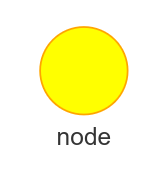
\includegraphics[width=0.7\textwidth]{figures/proposed_method/connecting_nodes/legend/node}
    \caption{Regular node created by the \ac{halgorithm}.\newline}%
    \end{subfigure}
    \begin{subfigure}{0.2\textwidth}
    \centering
    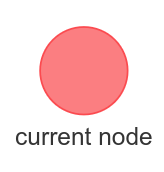
\includegraphics[width=0.7\textwidth]{figures/proposed_method/connecting_nodes/legend/current_node}
    \caption{Current node indicates that it's outgoing edge is or is next to be executed.}%
    \end{subfigure}
    \begin{subfigure}{0.2\textwidth}
    \centering
    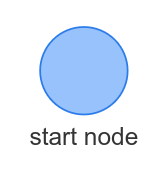
\includegraphics[width=0.7\textwidth]{figures/proposed_method/connecting_nodes/legend/starting_node}
    \caption{Starting node, one is generated at for every subtask.}%
    \end{subfigure}
    \begin{subfigure}{0.2\textwidth}
    \centering
    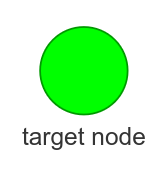
\includegraphics[width=0.7\textwidth]{figures/proposed_method/connecting_nodes/legend/target_node}
    \caption{Target node, one is generated for every subtask.\newline}%
    \end{subfigure}

    \begin{subfigure}{0.33\textwidth}
    \centering
    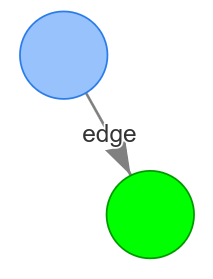
\includegraphics[width=0.7\textwidth]{figures/proposed_method/connecting_nodes/legend/edge}
    \caption{Edge with status IN, PE, SM, PP or EX.}%
    \end{subfigure}
    \begin{subfigure}{0.33\textwidth}
    \centering
    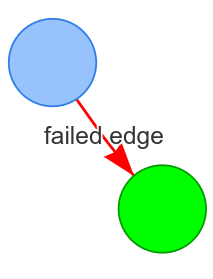
\includegraphics[width=0.7\textwidth]{figures/proposed_method/connecting_nodes/legend/failed_edge}
    \caption{Edge with status FAILED (FAIL)}%
    \end{subfigure}
    \begin{subfigure}{0.33\textwidth}
    \centering
    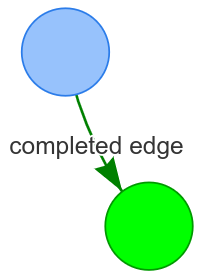
\includegraphics[width=0.7\textwidth]{figures/proposed_method/connecting_nodes/legend/completed_edge}
    \caption{Edge with status COMPLETED (CO)}%
    \end{subfigure}
    \caption{Legend for \ac{hgraph}'s nodes an edges}%
    \label{fig:hgraph_legend}
\end{figure}




This chapter has terminology that is conveniently grouped in the following table.

\noindent
\begin{table}[H]
\centering
\begin{tabular}%
  {>{\raggedright\arraybackslash}p{0.23\textwidth}%
   >{\raggedright\arraybackslash}p{0.67\textwidth}}
Task:   &  Tuple of objects and target configurations.\\
        & $\text{task} = \gls{task} = \left\langle \gls{Obj}_{\mathit{task}}, C_{\mathit{targets}} \right\rangle$\\
Subtask:& A single object, and a single target configuration.\\
        & $\text{subtask} = \gls{subtask}= \left\langle \mathit{obj}_{\mathit{subtask}}, \gls{c}_{\mathit{target}} \right\rangle$\\
Object Class & Classification assigned to an object.\\
             & $\gls{objectClass} = \textrm{Unknown}\vee \textrm{Obstacle}\vee \textrm{Movable}$\\
Node Status:& Status of a node indicates if a node is initialized, the \ac{halgorithm} was able to bring the object to the configuration or whether the \ac{halgorithm} fails to bring the object to its configuration.\\
            & \[\gls{nodeStatus} = \mathrm{Initialised} \vee \mathrm{Completed} \vee \mathrm{Failed} \]\\
Node:   & A node in the \acs{hgraph}, represents an object in a configuration with reachability indicated with a node status.\\
        & $\textrm{node} = \gls{node} = \left\langle \textrm{status}, \mathit{obj}, c \right\rangle$\\
Edge Status:& Status of a edge,\\
            & \[\gls{edgeStatus} = \mathrm{Initialised} \vee \mathrm{Path Exists} \vee \mathrm{System Model} \vee \] \[\mathrm{Path Planned} \vee \mathrm{Executing} \vee \mathrm{Completed} \vee \mathrm{Failed}\]\\
  & elaborate information on the edge statuses can be found in \Cref{tikz:status_action_edge}.\\
Edge:   & Edge connecting a node to another node in the \acs{hgraph} or \ac{kgraph}.\\
        & $ \textrm{edge} = \gls{edge} = \left\langle \textrm{status}, id_{\mathit{from}}, id_{\mathit{to}}, \textrm{verb}, \textrm{controller},\textrm{dynamic model}, \textrm{path}\right\rangle$\\
Hypothesis:& Sequence of successive edges in the \ac{hgraph}, an idea to put a object at it's target configuration. If executed and successfully completed, a subtask is completed.\\
           & $ \textrm{hypothesis} = \gls{hypothesis} = \left[\ \gls{edge}_{1}, \gls{edge}_{2}, \gls{edge}_{3}, \dots \gls{edge}_{m} \right]\ $, \hspace{0.5cm} $m>0$\\
Hypothesis Algorithm:& Graph based algorithm that searches for hypothesis in the \ac{hgraph} to complete subtasks eventually completing a task.\\
Hypothesis Graph:& Collection of nodes and edges. For every subtask a start and target node exist in the \ac{hgraph}, the \ac{halgorithm} searches for a path through nodes and edges to connect start to target node.\\
        & $ \textrm{\ac{hgraph}} = \gls{hgraph} = \left\langle \gls{nodesH}, \gls{edgesH} \right\rangle $\\
Knowledge Graph:& Collection of nodes and edges.  The \ac{kgraph} acts as a knowledge base and can be queried for an action suggestion.\\
        & $ \textrm{\ac{kgraph}} = \gls{kgraph} = \left\langle \gls{nodesK}, \gls{edgesK} \right\rangle $\\
\end{tabular}
\caption{Terminology of terms used}
\label{table:proposed_method_terminology}
\end{table}


